
\documentclass[twocolumn]{article}
\usepackage{mathpazo}
\usepackage{microtype}
\usepackage{times}
\usepackage{titlesec} % 1
\usepackage[colorlinks = true,
            linkcolor = blue,
            urlcolor  = blue,
            citecolor = blue,
            anchorcolor = blue]{hyperref}
%\usepackage{sectsty} % "제 1 절" ...

 %%%%%%%%%%%%%%%%%%%%%%%%%%%%%%%%%%%%%%%%%%%%%%%%%%%%%%%%%%%%%%%%%%%%%%%%%%%%%
 %                              My Commands
\newcommand{\bi}{\begin{itemize}}
\newcommand{\ei}{\end{itemize}}
\newcommand{\be}{\begin{enumerate}}
\newcommand{\ee}{\end{enumerate}}
\newcommand{\ii}{\item}
\newtheorem{Def}{Definition}
\newtheorem{Lem}{Lemma}
\usepackage{algorithm}
\usepackage{algorithmicx}
\usepackage{algpseudocode}

\usepackage{graphicx}
\graphicspath{%
        {converted_graphics/}
        {./images/}
}

\usepackage{color}
\usepackage{xcolor}
\usepackage{listings}
\usepackage{caption}
\DeclareCaptionFont{white}{\color{white}}
\DeclareCaptionFormat{listing}{\colorbox{gray}{\parbox{\textwidth}{#1#2#3}}}
\captionsetup[lstlisting]{format=listing,labelfont=white,textfont=white}
\usepackage{verbatimbox}

\usepackage[hangul,nonfrench,finemath]{kotex}
    
\setlength\textwidth{7in} 
\setlength\textheight{9.5in} 
\setlength\oddsidemargin{-0.25in} 
\setlength\topmargin{-0.25in} 
\setlength\headheight{0in} 
\setlength\headsep{0in} 
%\setlength\columnsep{5pt}
\sloppy 
 
\begin{document}

\title{
\vspace{-0.5in}\rule{\textwidth}{2pt}
\begin{tabular}{ll}\begin{minipage}{4.75in}\vspace{6px}
\noindent\large {\it KIWI Project}@Data Management Research Section\\
\vspace{-12px}\\
\noindent\LARGE ETRI\qquad  \large Technical Report 15ZS1410-TR-65
\end{minipage}&\begin{minipage}{2in}\vspace{6px}\small
218 Gajeong-ro, Yuseong-gu\\
Daejeon, 305-700, South Korea\\
http:/$\!$/www.etri.re.kr/\\
http:/$\!$/sungsoo.github.com/\quad 
\end{minipage}\end{tabular}
\rule{\textwidth}{2pt}\vspace{0.25in}
\LARGE \bf 국외 출장 보고서 \\
\large The International Conference on High Performance Computing \& Simulation (HPCS 2015)
}

\date{}

\author{
{\bf Sung-Soo Kim}\\
\it{sungsoo@etri.re.kr}
}

\maketitle

\begin{abstract}
현재까지 하둡과는 별개로 GPGPU기반 데이터관리 사례로는 하버드와 MIT에서 개발한 대규모 스트림데이터 처리/분석/가시화를 수행할 수 있는 시스템인 
GPGPU를 통해 하둡기반 빅 데이터 시스템의 성능을 높이기 위해서는 GPU상에서 다루어야 할 \textit{데이터 저장/압축모델}, \textit{처리 방식} 뿐만 아니라, \textit{질의 처리} 방식도 GPU에 최적화되어야 한다.
\end{abstract}

\section{본론}

\subsection{Keynote Presentation}
슈퍼컴퓨팅 변화에 대한 소프트웨어 변화전략, GPU 기반 클라우드 가속화 기술, e-Science를 위한 복합 e-Infrastructure, 유럽지역의 컴퓨팅 인프라 및 로드맵인  EGI-Engage등 4개 주제로 키노트 발표가 있었다. 본 절에서는 슈퍼컴퓨팅 변화에 대한 소프트웨어 변화전략과 GPU 기반 클라우드 가속화 기술에 대한 키노트 발표에 대해 기술한다.

\subsubsection{Architecture-aware Algorithms and Software for Peta and Exascale Computing}
\textbf{Speaker:} Jack Dongarra\\
University of Tennessee and Oak Ridge National Lab, Tennessee, USA; University of Manchester, U.K.

\noindent
\textbf{Contributions:} 본 키노트 발표에서는 지난 10년 동안 고성능 컴퓨팅 기술 변화에 대해 살펴보고, 주요 기술 동향에 따른 미래 예상되는 HPC 기술들에 대해 설명해 주었다. 그림 \ref{fig:hpc_20}은 지난 20년간 HPC 성능개발 변화 추이를 그래프이다. 현재 아이폰은 20년전 슈퍼컴퓨터의 성능과 동일함을 알 수 있다. 하지만, 발표자는 이러한 하드웨어 성능 개선속도에 비해 소프트웨어 변화가 더딘면이 있다고 지적했다.

\begin{figure}[htb]
        \centering
        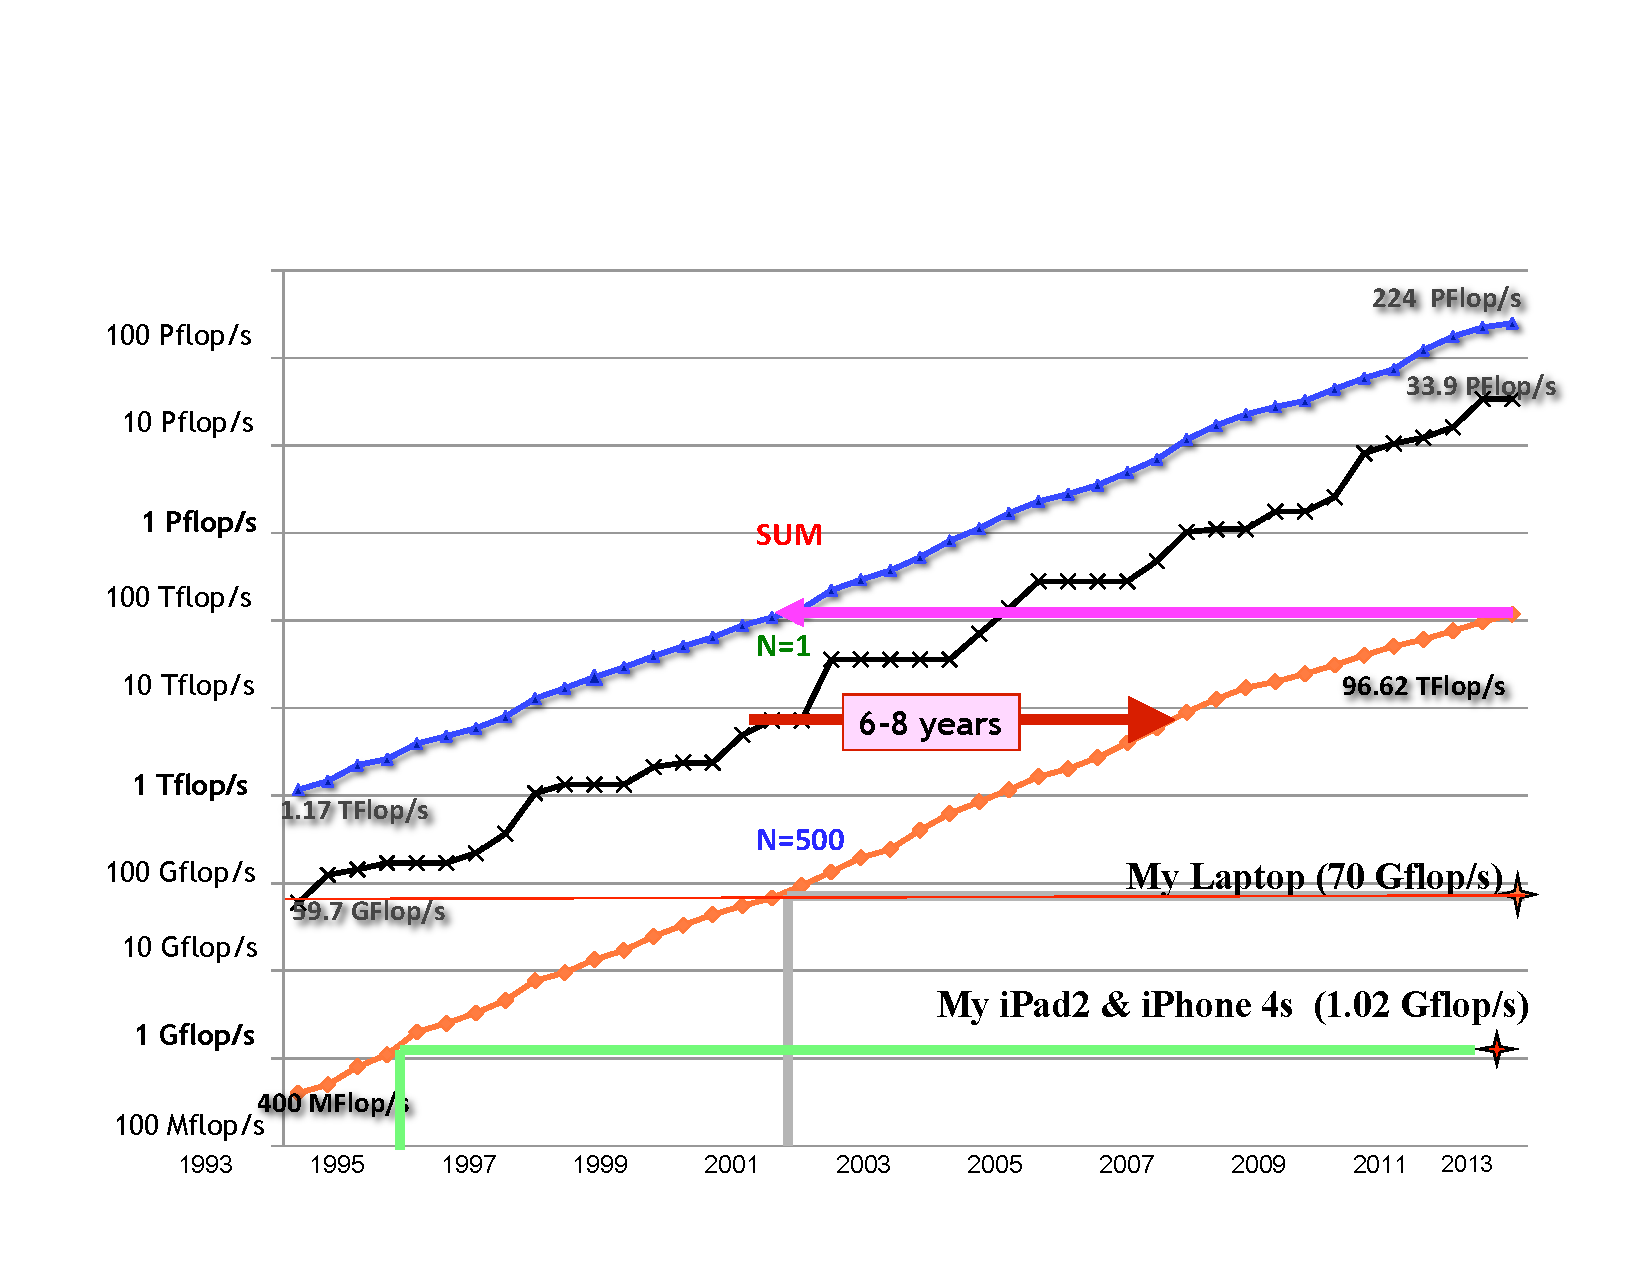
\includegraphics[width=0.48\textwidth]{hpc-20-years.pdf}
        \caption{Performance development of HPC over the last 20 years.}
        \label{fig:hpc_20}
\end{figure}
\noindent
\textbf{Why:}  지난 20년간 HPC 분야는 하드웨어 측면만을 지나치게 강조해서 연구개발 투자가 이루어져 왔다. HPC 기술 및 패러다임 변화는 우리가 개발하는 소프트웨어에 큰 영향을 미치기 때문에, HPC 기술이 어떻게 진화해 왔는지 그리고 앞으로 어떤 기술변화가 일어날 것인가 예측하는 것은 매우 중요하다. 현재 Top500의 99\% 시스템은 멀티코어 기반의 시스템이라고 한다. 따라서, 이러한 하드웨어 시스템 변화에 대응하는 소프트웨어 변화가 필요하다. 그림 \ref{fig:hpc_cores}는 슈퍼컴퓨터당 평균 코어수 변화 추이를 보여주고 있다.

\begin{figure}[htb]
        \centering
        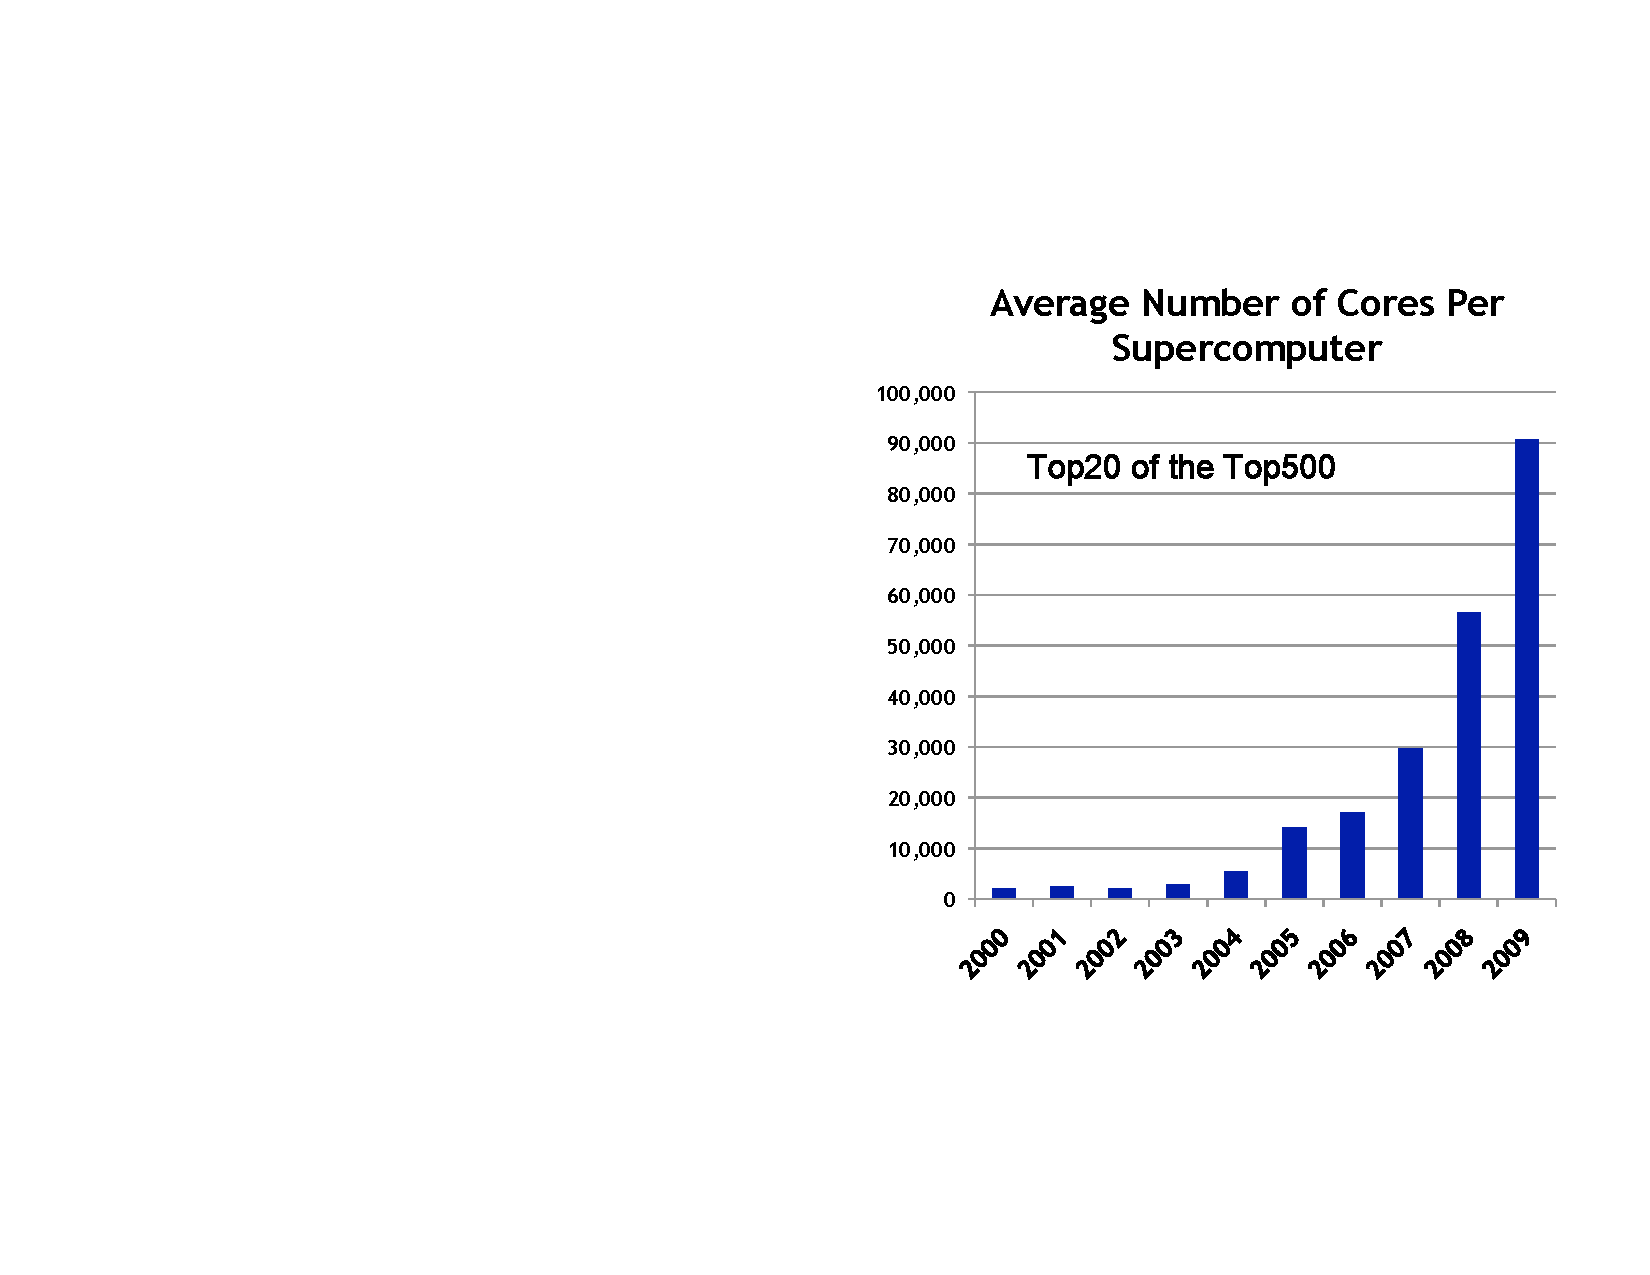
\includegraphics[width=0.48\textwidth]{hpc_cores.pdf}
        \caption{Average number of cores per supercomputer.}
        \label{fig:hpc_cores}
\end{figure}

\noindent
\textbf{How:}  소프트웨어 및 알고리즘 개발에 영향을 미칠 주요한 다섯가지 연구영역으로 나누어 기술변화를 예측하였다.
\bi
\ii 멀티코어 및 하이브리드 아키텍쳐에 맞게 소프트웨어 재설계 
\ii 자동 조정되는 응용 소프트웨어
\ii  성능을 위한 혼합 정밀도 활용하기
\ii 내고장성의 중요성
\ii 통신 회피 알고리즘
\ei

\noindent
\textbf{What:} Exascale computing으로 진화해 나가고 있는 HPC 하드웨어 및 소프트웨어 기술은 다음과 같다.
\bi
\ii Large-scale optics based interconnects
\ii Hardware and software based fault management
\ii Heterogeneous cores
\ii Another \textit{disruptive} technology
\bi
\ii Similar to what happened with \textit{cluster computing} and \textit{message passing}
\ei
\ei

\subsubsection{The Accelerated Cloud}
\textbf{Speaker:} Marc Hamilton\\
Vice President, Solutions Architecture and Engineering, NVIDIA, California, USA
\begin{figure}[htb]
        \centering
        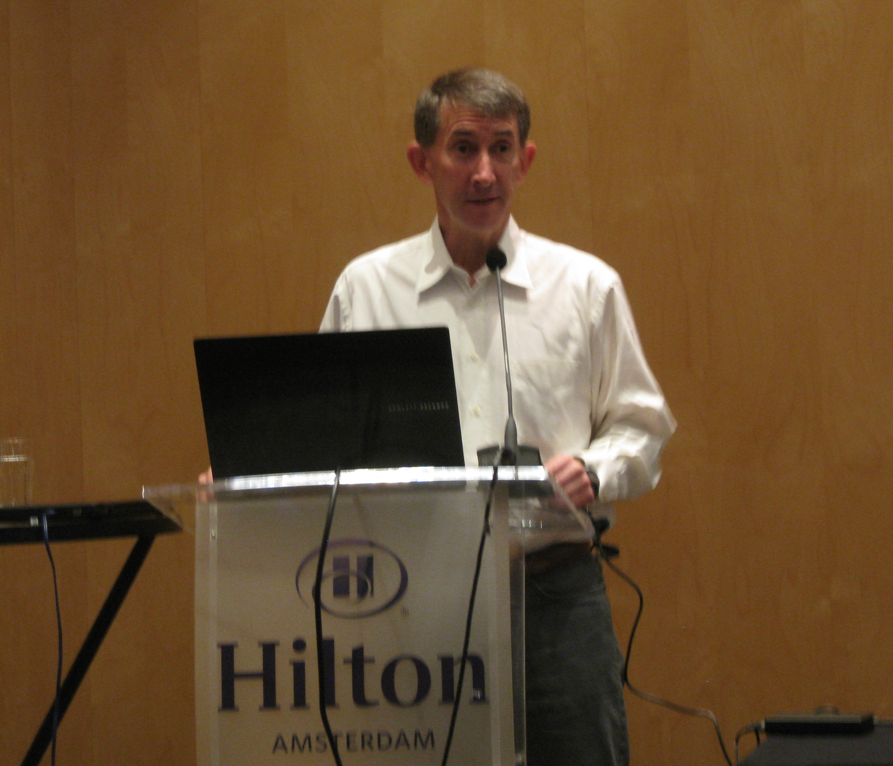
\includegraphics[width=0.45\textwidth]{marc.png}
        \caption{Marc Hamilton, NVIDIA}
        \label{fig:marc}
\end{figure}

\noindent
\textbf{Contributions:}  NVIDIA의 Marc Hamilton 기술이사 (그림 \ref{fig:marc})가 발표한 키노트는 
클라우드 컴퓨팅 및 HPC 기술 변화에 대해 살펴보고, NVIDIA의 GPU기반 클라우드 컴퓨팅 기술들에 대해 설명해 주었다. 
그림 \ref{fig:accelerated-data-center}은 GPU가 클라우드 컴퓨팅에 필요한 현재와 미래 유즈케이스를 보여 주고 있다.
구글은 공개적으로 내부 클라우드에 있는 GPU 1000대를 이용하여 40개의 GPU 가속 어플리케이션을 실행했다고 주장했다.
또한, 기계학습의 전문가인 Andrew Ng는 \textit{"향후 5년 내에, 50\%의 질의를 위해 사용되는 입력은 음성 또는 이미지다"} 라고 말했다.
이와 같이, GPU 기반 클라우드 컴퓨팅을 가속하기 위하여 NVIDIA는 주요 병목이였던 PCIe 버스 속도를 5배 개선한 NVLink 기술을 제공하고 있다고 한다.

\begin{figure}[htb]
        \centering
        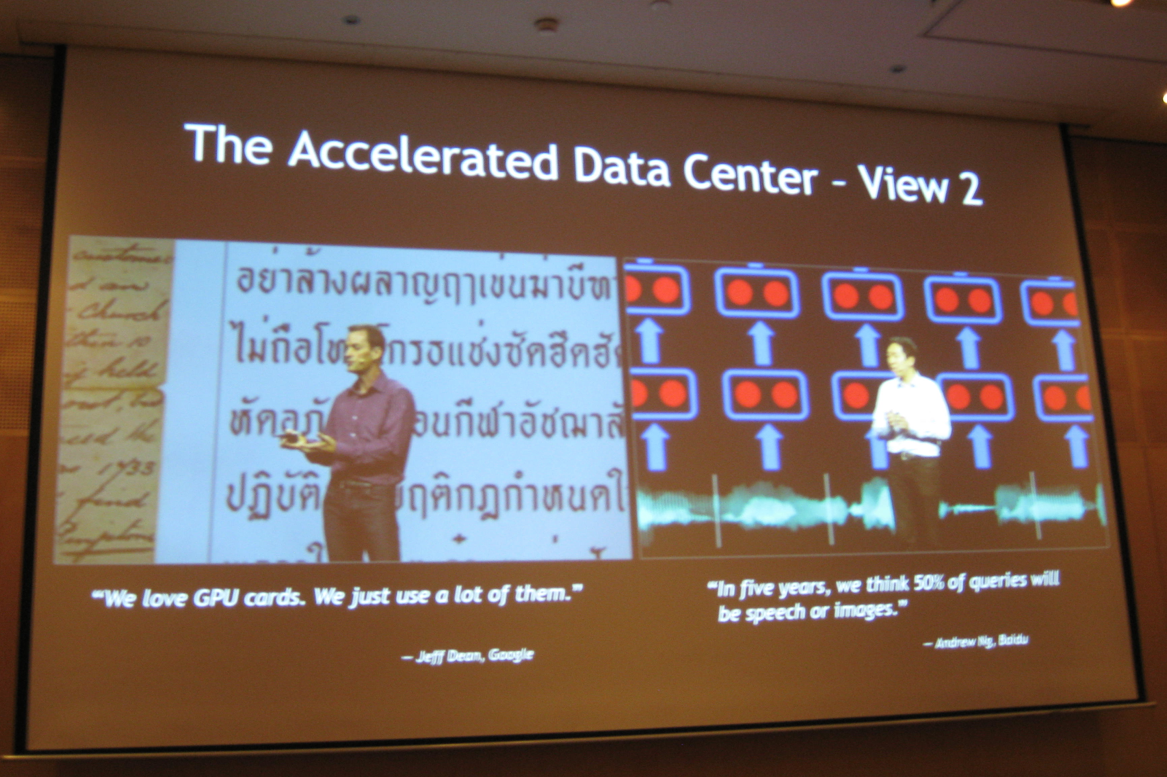
\includegraphics[width=0.48\textwidth]{marc-ppt.png}
        \caption{The Accelerated Data Center - View}
        \label{fig:accelerated-data-center}
\end{figure}

\noindent
\textbf{Technology Trends:}  가트너 (Gartner)의 서버 기술에 대한 2015년 하이퍼 사이클 \cite{George:2015}에 따르면, 신경망 실리콘 (\textit{Neural network silicon})이 대규모 데이터 병렬성을 가지는 문제를 해결하는 GPU 기반 하드웨어 가속화 기술이 이와 연관된다. 신경망 실리콘은 하이퍼 사이클상에서 현재(2015년 7월) 뜨는(on rise) 기술이며, 5년에서 10년사이에 정체기(plateau)에 접어들 것으로 가트너는 예상했다.
\begin{figure*}[htb]
        \centering
        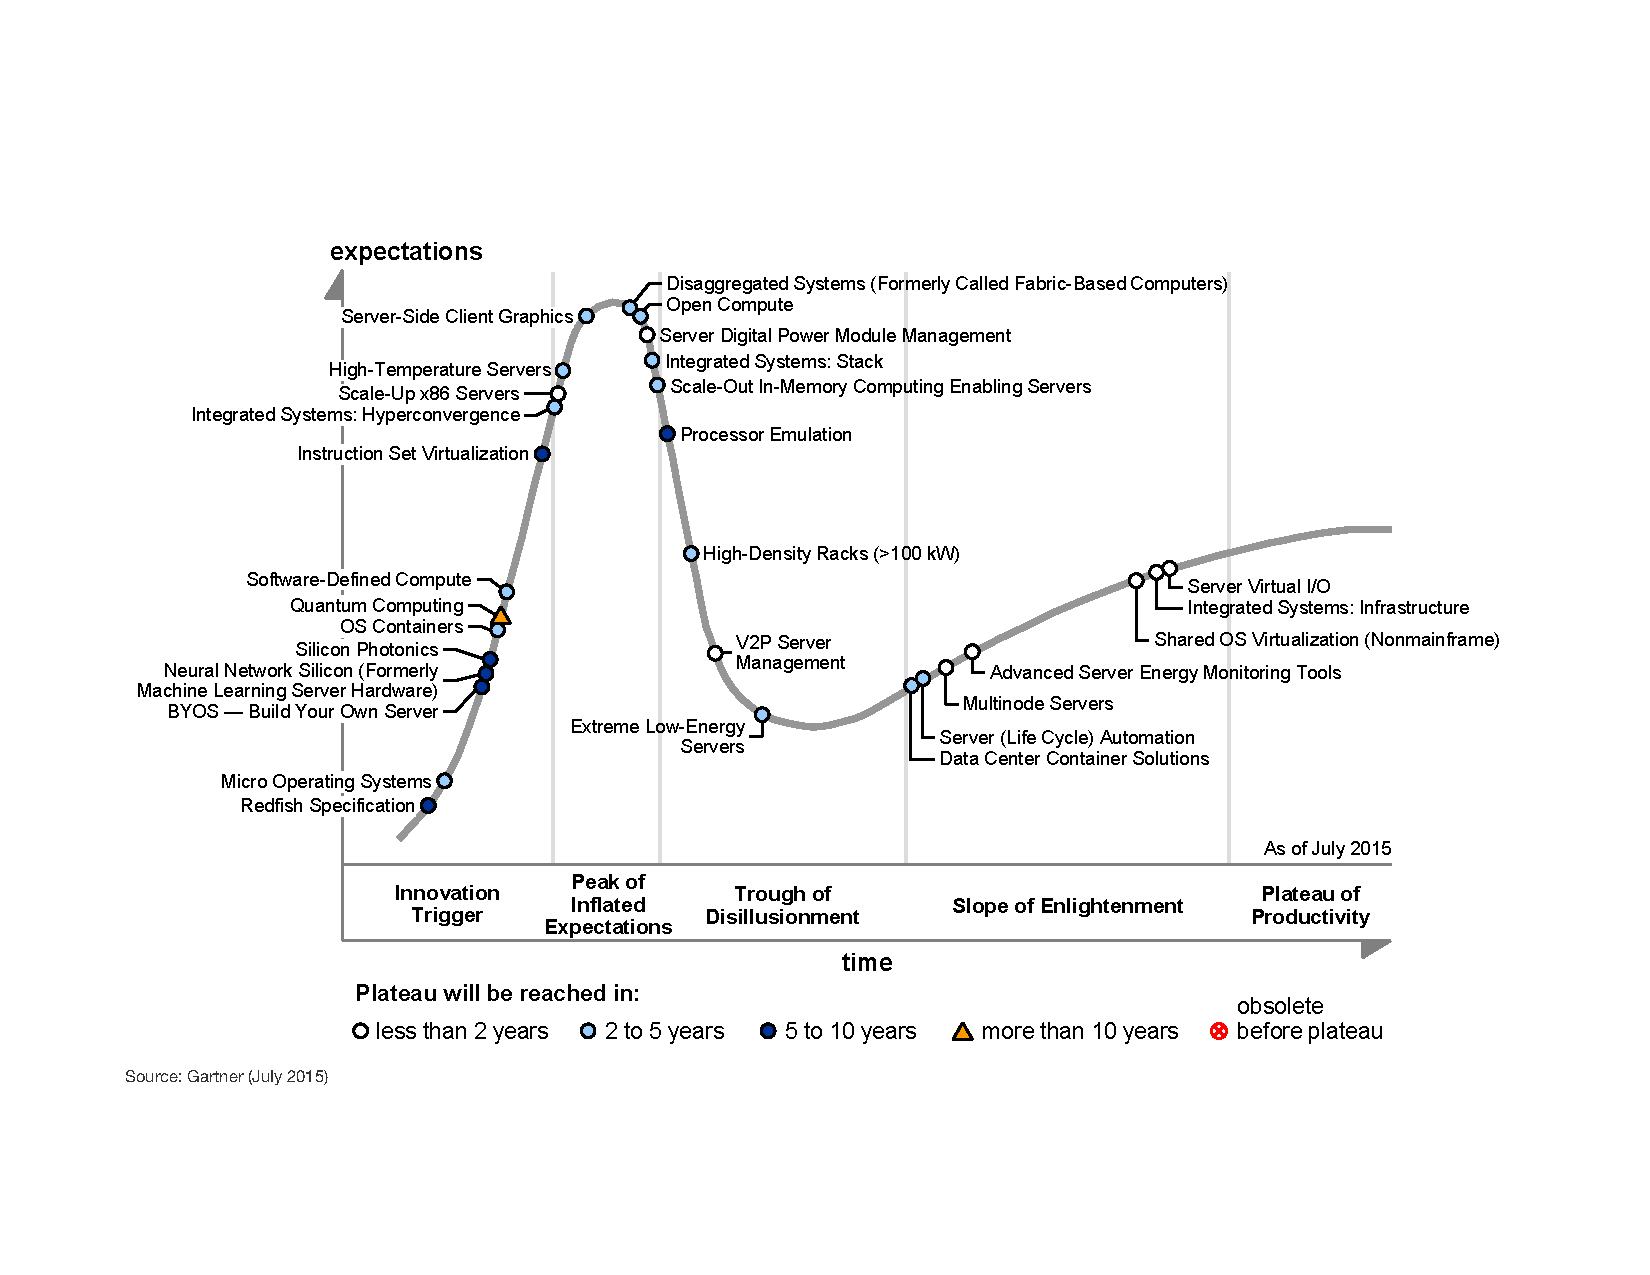
\includegraphics[width=1.0\textwidth]{gartner-server.pdf}
        \caption{Hype Cycle for Server Technologies, 2015 \cite{George:2015}}
        \label{fig:accelerated-data-center}
\end{figure*}
\bi
\ii \textbf{Neural Network Silicon:} 신경망 실리콘은 크게 깊은 신경망 (DNN; Deep Neural Network)을 이용한 기계학습 알고리즘의 성능을 향상 시킬수 있는 서버 기반 하드웨어 가속기를 의미한다. 
\ei
2012년 구글의 연구진은 DNN 기계학습 알고리즘을 GPU에 적용하여, 대규모 데이터 셋에 대한 학습시간(training time)을 획기적으로 단축시켰다고 한다.
또한, 모바일 장치 음성 인식과 웹 이미지 태깅에서 최근 개선들은 이러한 혁신과 직결된다고 볼 수 있다.

\noindent
\textbf{Why:}  전력 소비량은 HPC 시스템 운영에 있어서 중요한 이슈중에 하나다. 딥 러닝 (Deep learning)과 같은 대규모 데이터 병렬성이 요구되는 문제에는 GPU 하드웨어 자원을 이용하는 것이 전력 소비량에서 효과적이다. 다시 말해, GPU 기반 클라우드 컴퓨팅 및 데이터 센터는 수행 성능을 개선하면서 전력 소모 비용을 감축시킬 수 있는 방법이다.

\noindent
\textbf{How:}  NVIDIA는 GPU를 활용하여 데이터센터 및 클라우드 컴퓨팅의 성능 개선에 필요한 두가지 방법을 제공하고 있다.
첫 번째 방법은 기존의 CPU와 GPU사이의 PCIe 버스 병목을 해소하기 위한 방법으로 NVLink 기술을 제공한다.
두 번째 방법으로 CUDA 프로그래머를 위해 통합 메모리 (unified memory) 접근 기법과 고수준의 병렬 코드를 위한 프로그래밍 도구를 제공하는 것이다. 예를 들어,  동일한 C++ 코드를 NVIDIA GPU 코드, x86, ARM 그리고 Power CPU 코드로 변환 할 수 있는 Thrust 라이브러리를 제공한다.
이러한 두가지 방법을 지원하는 새로운 GPU 아키텍쳐인 파스칼 (Pascal) 아키텍쳐를 소개했다.

\begin{figure}[htb]
        \centering
        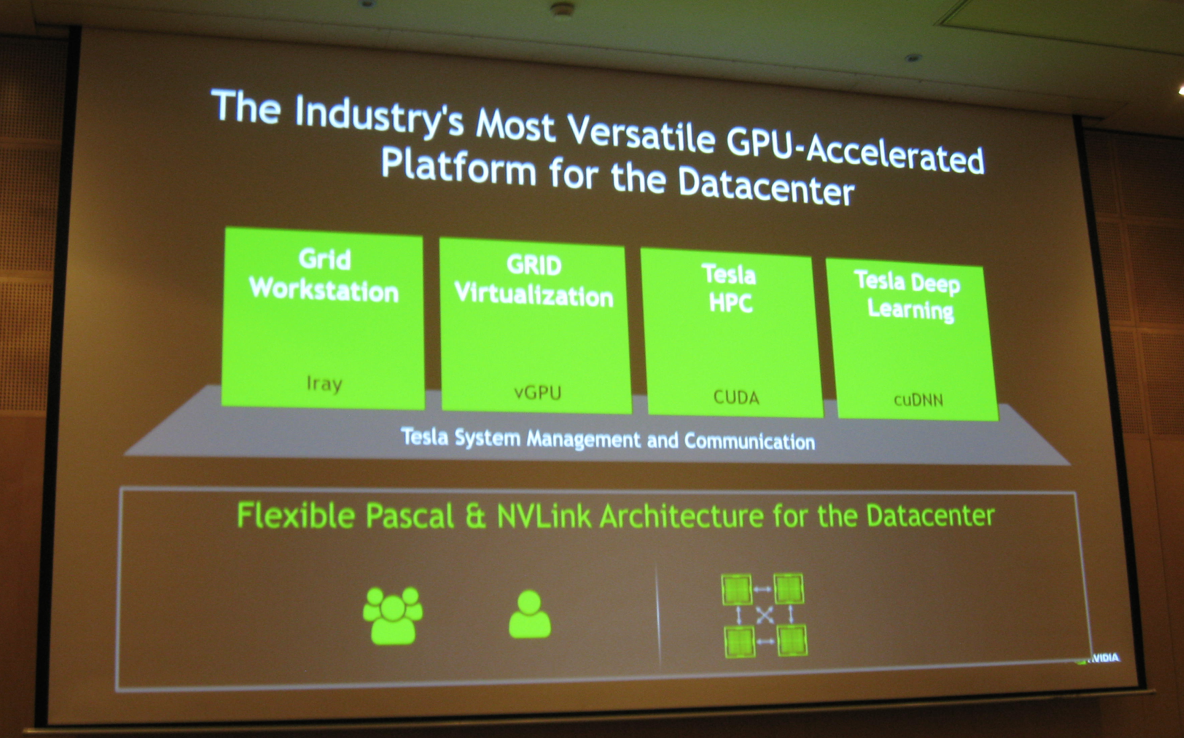
\includegraphics[width=0.48\textwidth]{gpu-platform.png}
        \caption{The industry's most versatile GPU-accelerated platform for the datacenter}
        \label{fig:gpu-accelerated-data-center}
\end{figure}

\noindent
\textbf{What:}  NVIDIA는 데이터 센터의 성능을 개선하기 위해 그림 \ref{fig:gpu-accelerated-data-center}과 같은 GPU 가속 기술을 적용한 플랫폼을 구축하여 운영하고 있다.
\bi
\ii Grid Workstation (Iray)
\ii GRID Virtualization (vGPU)
\ii Tesla HPC (CUDA)
\ii  Tesla Deep Learning (cuDNN)
\ii Tesla System Management and Communication
\ii  Flexible Pascal \& NVLink Architecture for the Datacenter: 파스칼 GPU는 170억개의 트랜지스터와 32GB VRAM을 갖추고 있다. (그림 \ref{fig:gpu-architecture})
\ei

\begin{figure}[htb]
        \centering
        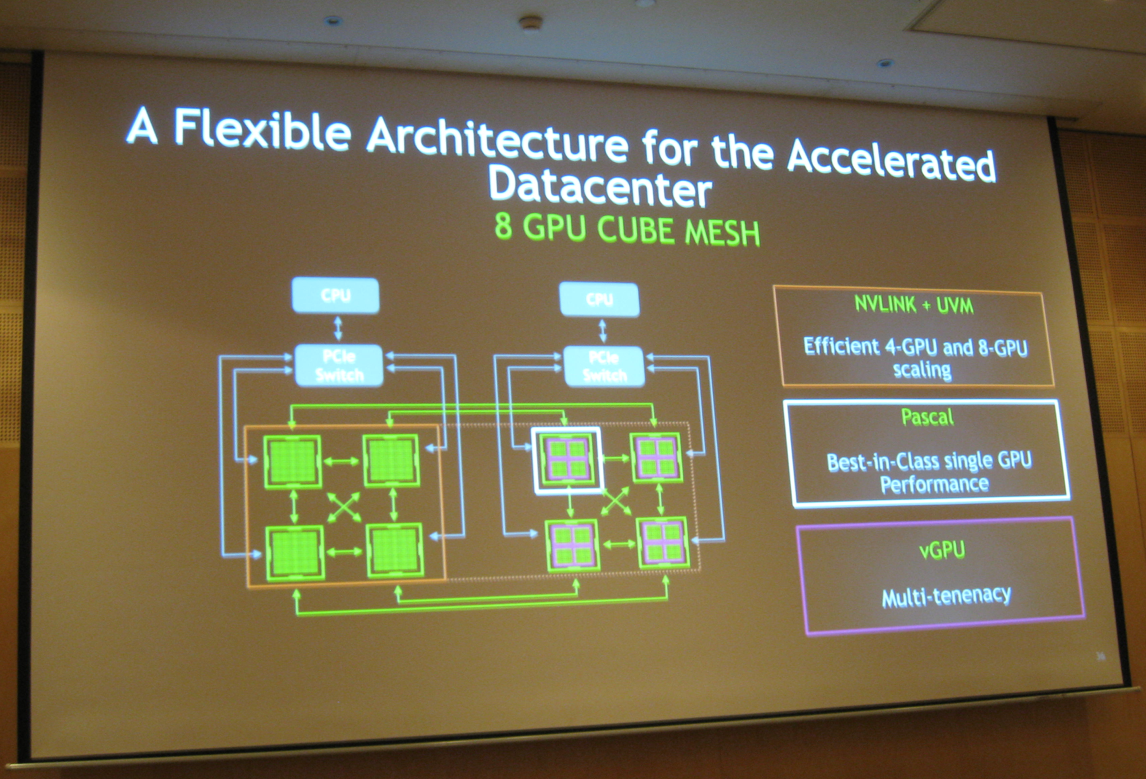
\includegraphics[width=0.48\textwidth]{gpu-architecture.png}
        \caption{A flexible architecture for the accelerated datacenter}
        \label{fig:gpu-architecture}
\end{figure}

\section{Paper Sessions}
\subsection{GENERAL PURPOSE GRAPHICS PROCESSING UNITS (GPGPU): : ACCELERATION, ALGORITHMS AND PERFORMANCE}

\subsubsection{A Runtime/Memory Trade-off of the Continous Ziggurat Method on GPUs}
\textbf{Speaker:} Christoph Riesinger (Technische Universitat Munchen, Munich, Germany)

\subsubsection{Cph CT Toolbox: A Performance Evaluation}
\textbf{Speaker:} Jonas Bardino (University of Copenhagen, Copenhagen, Denmark)

\subsubsection{Acceleration of dRMSD Calculation and Efficient Usage of GPU Caches}
\textbf{Speaker:} Jiri Filipovic (Masaryk University, Brno, Czech Republic)

\subsubsection{Optimizing Communications in multi-GPU Lattice Boltzmann Simulations}
\textbf{Speaker:} Sebastiano Fabio Schifano (Universita di Ferrara and INFN, Ferrara, Italy)

\subsection{HIGH PERFORMANCE MEMORY SYSTEMS AND DISTRIBUTED STORAGE AND WAREHOUSING}
\subsubsection{Analysis of Asymmetric 3D DRAM Architecture in Combination with L2 Cache Size Reduction}
\textbf{Speaker:} Alex Schoenberger (Technische Universität Darmstadt, Darmstadt, Germany)
\subsubsection{Tracing Long Running Applications: A Case Study Using Gromacs}
\textbf{Speaker:} Michael Wagner (Center for Information Services and High Performance Computing (ZIH), Technische Universitat Dresden, Dresden, Germany)
\subsubsection{Advanced Commands and Distributed Data Layout to Enhance the SSD Internal Parallelism}
\textbf{Speaker:} Soraya Zertal (PRiSM, Université de Versailles, Versailles, France)

\subsection{HPCS 2015 POSTER PAPERS}
\be
\ii Real-time Signal Identification in Big Data Streams Bragg–Spot Localization in Photon Science
\ii A Resilient Routing Approach for Mobil Ad Hoc Networks
\ii Efficient Asian Option Pricing with CUDA
\ii GPGPU Performance Evaluation of Some Basic Molecular Dynamics Algorithms
\ii Cookery: A Framework for Developing Cloud Applications
\ii Subordination: Cluster Management without Distributed Consensus
\ee

\subsection{HIGH PERFORMANCE MOBILE ARCHITECTURES, WIRELESS NETWORKS AND APPLICATIONS}
\subsubsection{GPU Accelerated Ray Launching for High-Fidelity Virtual Test Drives of VANET Applications}
\textbf{Speaker:} Manuel Schiller, (Lehrstuhl fur Echtzeitsysteme und Robotik, Technische Universitat Munchen, Germany)
\subsubsection{A Collaboration Middleware for Service Scalability in Peer-to-Peer Systems}
\textbf{Speaker:} Sung-Soo Kim (ETRI, Daejeon, South Korea)
\subsubsection{Experiments in Fair Scheduling in 4G WiMAX and LTE}
\textbf{Speaker:} Junaid Ahmed Zubairi (State University of New York at Fredonia, New York, USA)

\subsection{IMAGE PROCESSING, MACHINE LEARNING, PATTERN RECOGNITION \& APPLICATIONS}

\subsubsection{A Reduced Complexity Instruction Set Architecture for Low Cost Embedded Processors}
\textbf{Speaker:} Mabo Ito (The University of British Columbia - Vancouver, British Columbia, Canada)

\subsubsection{Deep Learning with Shallow Architecture for Image Classification}
\textbf{Speaker:} Asma ElAdel (National School of Engineers of Sfax, Sfax, Tunisia)

\subsubsection{An Efficient Implementation of Fuzzy Edge Detection Using GPUs in MATLAB}
\textbf{Speaker:} Farnaz Hoseini (Islamic Azad University, Rasht, Iran; University of Guilan, Rasht, Iran)

\subsection{RESOURCE ALLOCATION, SCHEDULING, AND LOAD BALANCING IN HPC SYSTEMS}
\subsubsection{Market-inspired Dynamic Resource Allocation in Many-core High Performance Computing Systems}
\textbf{Speaker:} Amit Kumar Singh (University of York, York, U.K.)
\subsubsection{234 Scheduling of 3-2 and 2-1 Eliminations for Parallel Image Compositing using Non-Power-of-Two Number of Processes}
\textbf{Speaker:} Jorji Nonaka (RIKEN Advanced Institute of Computational Science, Kobe, Japan; Light Transport Entertainment, Inc., Tokyo, Japan)
\subsubsection{In Search of the Best MPI-OpenMP Distribution for Optimum Intel-MIC Cluster Performance}
\textbf{Speaker:} Gladys Utrera (Universitat Politecnica de Catalunya-Barcelona, Barcelona, Spain)

% Example Figure
%%%%%%%%%%%%%
%\begin{figure}[htb]
%        \centering
%        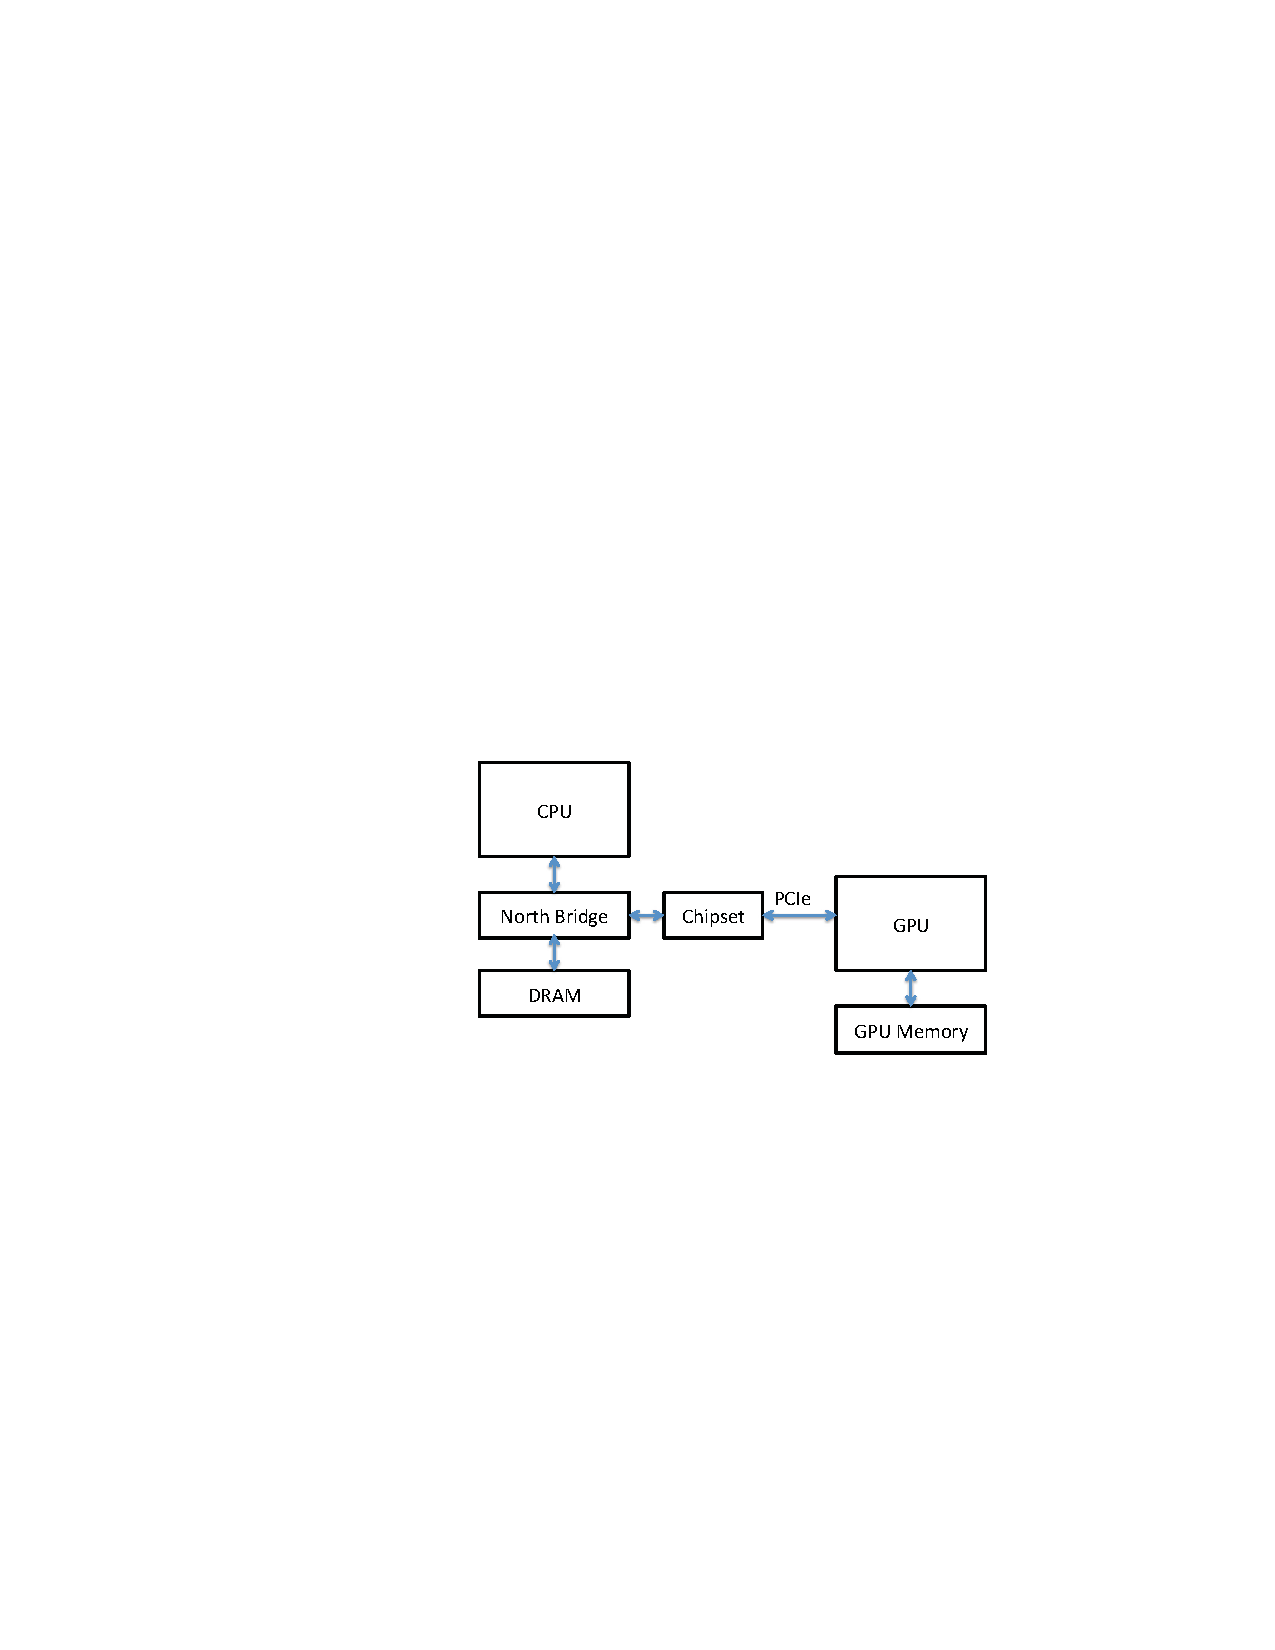
\includegraphics[width=0.48\textwidth]{system-overview.pdf}
%        \caption{A system overview with CPU and a discrete GPU.}
%        \label{fig:system_overview}
%\end{figure}



\bibliographystyle{abbrv}
\bibliography{sqlonhadoop}

\end{document}
